% ============================ Enrico Ribiani 16-03-2021 ====================================================================
% Base per i documenti  
\documentclass[12pt]{article}
% ------------ pacchetti necessari ----------------
\usepackage[a4paper, total={6in, 8in},margin=1in]{geometry} % formattazione decente della pagina
\usepackage{graphicx}                            % need for figure
\usepackage{amsmath}
\usepackage{amsfonts}                            % if you want the fonts
\usepackage{amssymb}                             % if you want extra symbols
\usepackage{graphicx}  
\renewcommand{\figurename}{Figura}  
\renewcommand{\contentsname}{Indice}                        % need for figures
\usepackage{mathptmx}
\usepackage{float}                               % serve per mettere tabelle e immagini dove si vuole 
\usepackage[utf8]{inputenc}
\usepackage{textcomp}
\usepackage[hang,flushmargin,bottom]{footmisc}   % footnote format
\usepackage{fancyhdr, lastpage}
\usepackage{titlesec}
\usepackage[table,dvipsnames]{xcolor}
%\pagestyle{fancy}
%\renewcommand{\headrulewidth}{0pt}
%\renewcommand*\contentsname{Indice}
\titleformat{\section}{\normalsize\bfseries}{\thesection.}{1em}{}	% required for heading numbering style
\titleformat*{\section}{\Large\bfseries}
\titleformat*{\subsection}{\large\bfseries}
%\usepackage{siunitx}
%\usepackage{tikz}
\usepackage{circuitikz}
%\usepackage[siunitx]{circuitikz}
\usepackage{multirow}
\usepackage{tikz}
\usepackage{amsmath}
\usetikzlibrary{angles,quotes}
\usepackage{placeins}
\usepackage{multirow}
%===================links=================
\usepackage{hyperref}
\hypersetup{
    colorlinks=true,
    linkcolor=Sepia,
    filecolor=Green,      
    urlcolor=Cyan,
    pdftitle={SAMPLE},
    pdfpagemode=FullScreen,
    }
    \usepackage{kvoptions}
    \usepackage{xcolor-material}
    \definecolor{nred}{RGB}{191, 97, 106}
    \definecolor{norange}{RGB}{208, 135, 112}
    \definecolor{nyellow}{RGB}{163, 190, 140}
    \definecolor{ngreen}{RGB}{35, 203, 139}
    \usepackage{colortbl}
    \usepackage{nicematrix}
%===================inizio pagina del titolo=================
\begin{document}
    \begin{titlepage}
    \begin{center}
% ------------------ inizio immagine logo ----------
\begin{figure}
    \centering
    
\includegraphics{~/varie/logo.png}
    \label{fig:logo}
\end{figure}
% ------------------ fine immagine logo ----------
% ------------------ fine immagine logo ----------
-------------------------------------------------------------------------------------\\
\vspace{2\baselineskip}
\large Enrico Ribiani\\
\large 4AUB\\
\vfill

\Huge{\textbf{Esperienza laboratoriale diodi e limitatori}}\\
\vfill

\LARGE{esperienza n°4}\\
\vfill
\large{24-11-2021}
\end{center}
%=============== fine pagina titolo ===============
\end{titlepage}
\tableofcontents
\vskip 1cm
\section{Scopo:Verificare sperimentalmente la curva caratteristica di un diodo.}
    \subsection{Materiale}
    \begin{itemize}
        \item resistenza da 2,2k$\Omega$
        \item resistenza da 1k$\Omega$
        \item diodo [codice prodotto]
        \item 2x diodo zener [codice prodotto]
       
        \item cavi per il collegamento
    \end{itemize}
    \subsection{Strumenti}
    \begin{itemize}
        \item alimentatore
        \item multimetro
        \item ocilloscopio
        \item generatore di funzione
    \end{itemize}
    \subsubsection{Schema}
    \begin{center}
        \begin{circuitikz}[european]
        \draw
          (0,0) to [short, *-] (6,0)
          %COME SI LEVA QUEL + - AAAAAAAAAAAAAAAAAA
          to [R, l_=$R_L$] (6,4) 
          to [short] 
          (5,4) 
          (0,0) to [open, v=E ] 
          (0,4) 
          to [short, *- ] 
          (1,4) 
          to [R, l=$R$] 
          (3,4)
          to (5,4) 
          to [short, i_=$i_d$] (5,3) 
          to [D, l_=$D$] (5,0); 
        \end{circuitikz}
        \end{center}
    \section{Cenni teorici}
    \subsection{Previsione comportamento}
    \section{Procedimento}
    \subsection{Tabelle} 
    \begin{table}[H]
        \begin{tabular}{|c|c|c|c|}
            \hline
            \rowcolor{RawSienna!80} E [V] & $V_r$[V] & $I_d=V_r/R [A]$ & $V_d=V-V_r$  \\
            \hline
            \rowcolor{Orange!70} 0 & 0 & 0  & 0 \\
            \hline
            \rowcolor{TealBlue!70} 0,5 & 0,0617 &  0,0000617 &  0,4383 \\
            \hline
            \rowcolor{Orange!70} 1 & 0,4632 &   0,0004632  &  0,5368 \\
            \hline
            \rowcolor{TealBlue!70} 1,5  & 0,9266 &   0,0009266  & 0,5734  \\
            \hline
            \rowcolor{Orange!70} 2 & 1,4036 & 0,0014036  & 0,5964  \\
            \hline
            \rowcolor{TealBlue!70} 2,5  & 1,8941 &  0,0018941   & 0,6059  \\
            \hline
            \rowcolor{Orange!70} 3 & 2,3805 & 0,0023805  & 0,6195  \\
            \hline
            \rowcolor{TealBlue!70} 3,5  & 2,8708 &   0,0028708  & 0,6292  \\
            \hline
            \rowcolor{Orange!70} 4 & 3,3604 & 0,0033604  & 0,6396  \\
            \hline
            \rowcolor{TealBlue!70} 4,5  & 3,8537 &   0,0038537  & 0,6463  \\
            \hline
            \rowcolor{Orange!70} 5 & 4,438 &  0,004438 & 0,655  \\
            \hline
            \rowcolor{TealBlue!70} 5,5  & 4,8492 &  0,0048492   &  0,659 \\
            \hline
            \rowcolor{Orange!70} 6 & 5,336 &  0,005336 &  0,664 \\
            \hline
            \rowcolor{TealBlue!70} 6,5  & 5,826 &  0,005826   & 0,671  \\
            \hline
            \rowcolor{Orange!70} 7 & 6,365 & 0,006365  & 0,675  \\
            \hline
            \rowcolor{TealBlue!70} 7,5  & 6,838 &   0,006838  &  0,006838 \\
            \hline
            \rowcolor{Orange!70} 8 & 7,324 &  0,007324 &  0,676 \\
            \hline
            \rowcolor{TealBlue!70} 8,5  & 7,841 &  0,007841   &  0,679 \\
            \hline
            \rowcolor{Orange!70} 9 & 8,314 & 0,008314  &  0,686 \\
            \hline
            \rowcolor{TealBlue!70} 9,5  & 8,818 &   0,008818  & 0,682  \\
            \hline
            \rowcolor{Orange!70} 10 & 9,311 & 0,009311  &  0,689 \\
            \hline
            \rowcolor{TealBlue!70} 10,5  & 9,311 &  0,009311   &  0,689 \\
            \hline
            \rowcolor{Orange!70} 11 & 10,308 &  0,010308 &  0,692 \\
            \hline
            \rowcolor{TealBlue!70} 11,5  & 10,811 &  0,010811   &0,693   \\
            \hline
            \rowcolor{Orange!70} 12 & 11,3 & 0,0113  & 0,694  \\
            \hline
        \end{tabular}
    \end{table}
    \subsection{Grafico}
    \begin{figure}[!h]
        \centering
        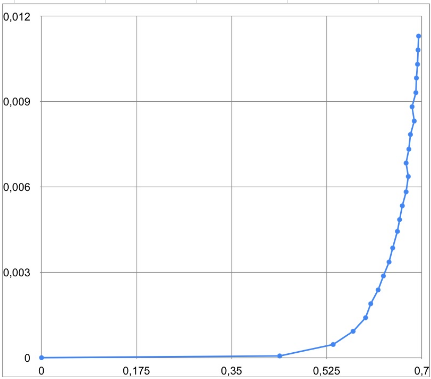
\includegraphics[scale=0.8]{media/graph.png}
        \caption{Grafico caratteristica IV del diodo,\\ V sulle ordinate, I sulle ascisse.}
    \end{figure}
    Possiamo osservare che nonostante qualche imprecisione data dal fatto che i componenti sono reali e questo comporta tutti gli 
    errori intrinseci, nonostante ciò si può osservare che il grafico rispetta la curva ideale del diodo, si può notare che la soglia $V_s$
    è intorno ai 5,25 V.\\
    \subsection{Calcoli}
    \section{Conclusioni}
\section{Osservazione circuiti limitatori}
\section{Foto}
    \end{document}
